% Short demo for \LaTeX beamer theme with ACON style layout
%
% Author: Thomas Meurer <tm@tf.uni-kiel.de>
% Version history:
% v0 ... 2016/12/09

\documentclass[10pt,t,aspectratio=1610]{beamer}
%\usetheme[german]{ACON} %or 
\usetheme{ACON}

% We define  a command \sfcite which enables to add citations but to
% preserve the citation number throughout the presentation. Citations
% are placed on the slide, where \sfcite is called. For the standard
% behavior of citations use \footcite.
%
% This also requires to add the following two lines to the main LaTeX
% source file:
%
\usepackage[style=numeric-comp,citetracker=true,sorting=none]{biblatex}
\bibliography{example}
\usepackage{abbreviations} %Provide an abbreviations file if equations
                          %are used
\usepackage{curve2e}

\usepackage{media9} %For Video Playback

% ### Changes by JW #################

% Some useful Packages
%\usepackage{enumitem}
\usepackage{circuitikz}

% New Commands
\setbeamerfont{title}{series=\bfseries,size={\fontsize{16}{16}}} % Title Font Size

\newcommand{\CustomShortTitle}{Eine Anwendung des Reinforcement Learning zur Regelung dynamischer Systeme} % Short-Title for Footer

% ------------------------------------

% Itemize Icons
\newcommand{\IconPro}{\raisebox{-1.5pt}{
\includegraphics[width=1em]{icons/001-plus.pdf}}}
\newcommand{\IconCon}{\raisebox{-1.5pt}{
\includegraphics[width=1em]{icons/002-minus.pdf}}}
\newcommand{\IconArrow}{\raisebox{-1.5pt}{
\includegraphics[width=1em]{icons/003-arrow.pdf}}}

\newcommand{\MotorNeuron}{\raisebox{-6pt}{\includegraphics[width=2em]{icons/motor_neuron.pdf}}}
\newcommand{\SensorNeuron}{\raisebox{-6pt}{\includegraphics[width=2em]{icons/sensor_neuron.pdf}}}
\newcommand{\InterNeuron}{\raisebox{-6.5pt}{\includegraphics[width=2em]{icons/inter_neuron.pdf}}}

% ------------------------------------
% Chapter and Section Names
\newcommand{\Inhalt}{Inhaltsübersicht}
\newcommand{\ChapterBnn}{Grundlagen biologischer neuronaler Netze}
\newcommand{\ChapterRl}{Reinforcement Learning - Lernen mit Belohnung}
\newcommand{\ChapterCartpole}{Implementierung und Simulation des inversen Pendels}
\newcommand{\ChapterEnd}{Zusammenfassung}

% ------------------------------------
% File Tree
\usepackage[edges]{forest} % For File-Trees
% Some Renewcommands for FOREST-------------------
\definecolor{folderbg}{RGB}{124,166,198}
\definecolor{folderborder}{RGB}{110,144,169}
\newlength\Size
\setlength\Size{4pt}
\tikzset{%
	folder/.pic={%
		\filldraw [draw=folderborder, top color=folderbg!50, bottom color=folderbg] (-1.05*\Size,0.2\Size+5pt) rectangle ++(.75*\Size,-0.2\Size-5pt);
		\filldraw [draw=folderborder, top color=folderbg!50, bottom color=folderbg] (-1.15*\Size,-\Size) rectangle (1.15*\Size,\Size);
	},
	file/.pic={%
		\filldraw [draw=folderborder, top color=folderbg!5, bottom color=folderbg!10] (-\Size,.4*\Size+5pt) coordinate (a) |- (\Size,-1.2*\Size) coordinate (b) -- ++(0,1.6*\Size) coordinate (c) -- ++(-5pt,5pt) coordinate (d) -- cycle (d) |- (c) ;
	},
}
\forestset{%
	declare autowrapped toks={pic me}{},
	pic dir tree/.style={%
		for tree={%
			folder,
			font=\ttfamily,
			grow'=0,
		},
		before typesetting nodes={%
			for tree={%
				edge label+/.option={pic me},
			},
		},
	},
	pic me set/.code n args=2{%
		\forestset{%
			#1/.style={%
				inner xsep=2\Size,
				pic me={pic {#2}},
			}
		}
	},
	pic me set={directory}{folder},
	pic me set={file}{file},
}
% ------------------------------------

% ####################################


\title{Eine Anwendung des Reinforcement Learning auf biologische neuronale Netze zur Regelung dynamischer Systeme am Beispiel des inversen Pendels}

\subtitle{Abschlussvortrag Bachelorarbeit}
\author[J. Wilinski]{Jonas Helmut Wilinski}
\pauthoremail{stu118261@mail.uni-kiel.de}
\institute[ACON]{Abschlussvortrag Bachelorarbeit, Kiel (Germany),}
\date{14. September 2018}
\begin{document}

% =======================

\begin{frame}[plain]
  \titlepage
\end{frame}

% =======================

\begin{frame}
\frametitle{\Inhalt}
\framesubtitle{Übersicht der Themen dieser Bachelorarbeit}
\vspace{1cm}
\begin{columns}[T,onlytextwidth]
	\begin{column}{0.3\textwidth}
		\centering
		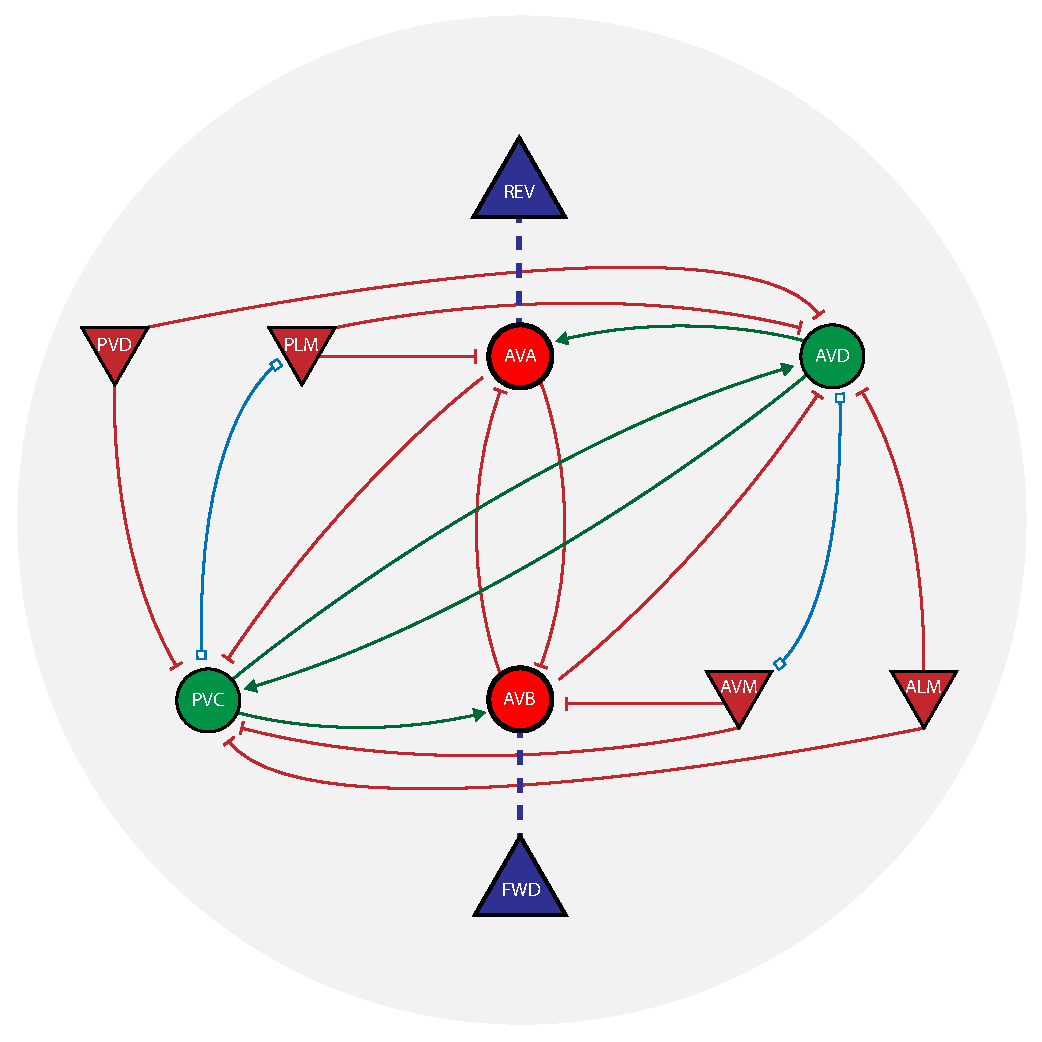
\includegraphics[width=4.5cm]{figures/folie_1/bnn.pdf}
		\btEmph{Biologische neuronale Netze}
	\end{column}
	\hspace{0.2cm}
	\begin{column}{0.3\textwidth}
		\centering
		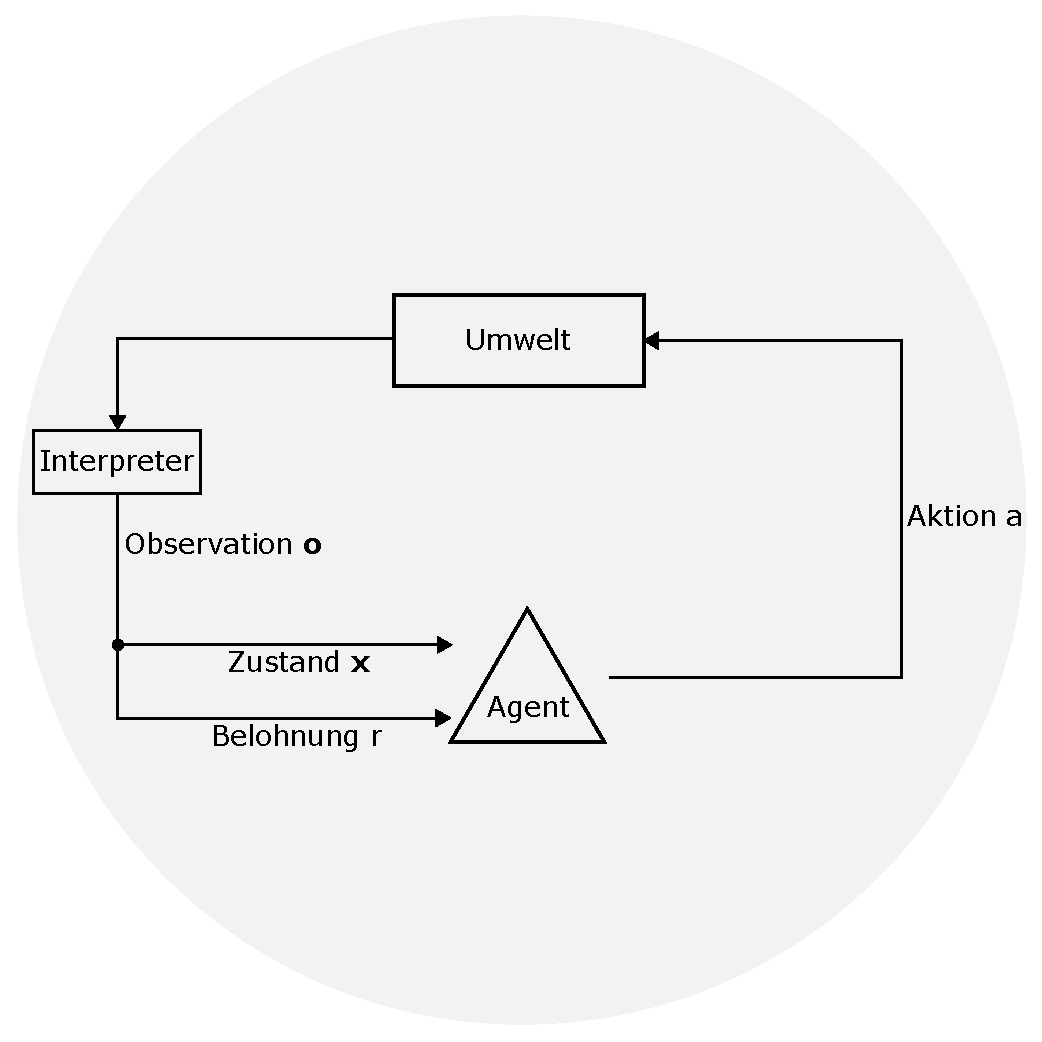
\includegraphics[width=4.5cm]{figures/folie_1/rl.pdf}
		\btEmph{Reinforcement Learning}
	\end{column}
	\hspace{0.2cm}
	\begin{column}{0.3\textwidth}
		\centering
		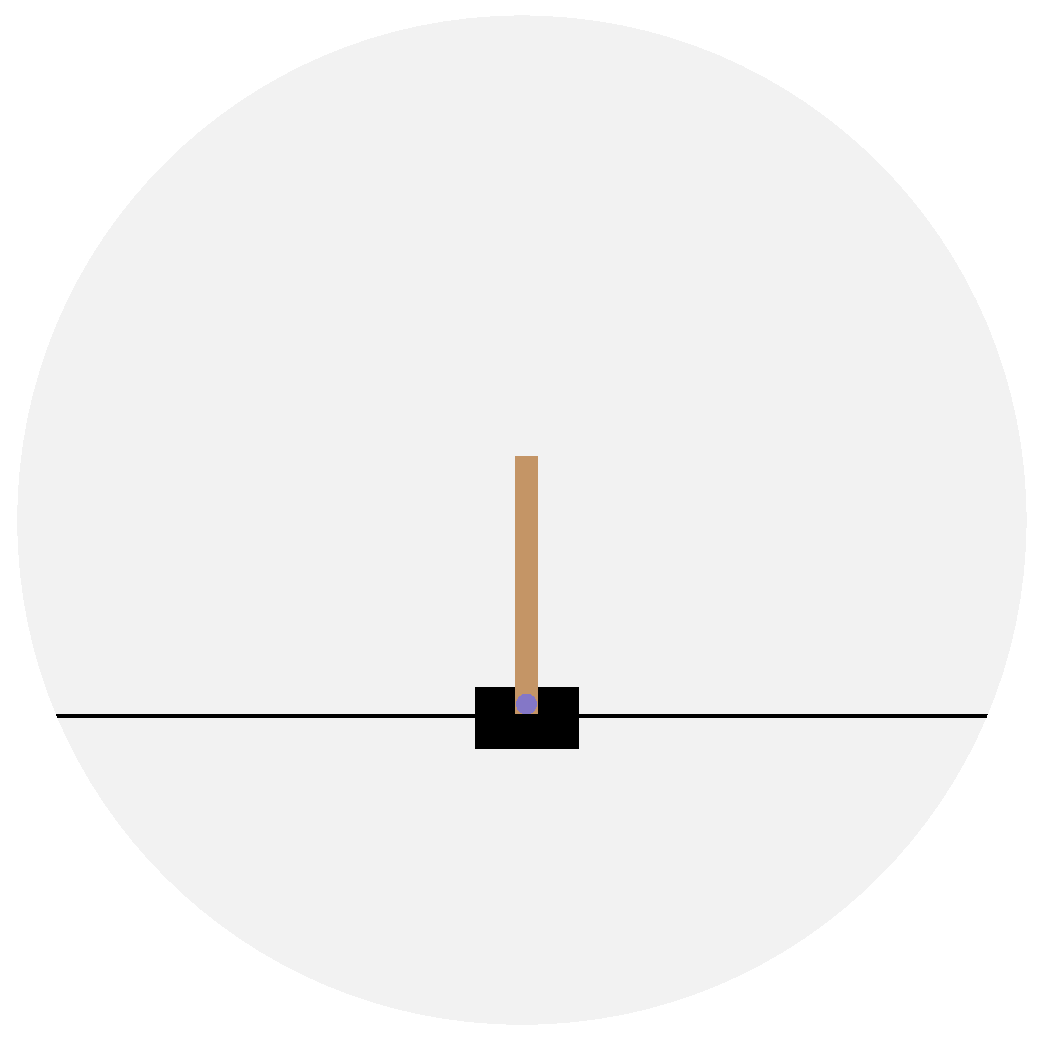
\includegraphics[width=4.5cm]{figures/folie_1/cartpole.pdf}
		\btEmph{Simulation: inverses Pendel}
	\end{column}
\end{columns}

\end{frame}

% =======================

\begin{frame}
	\frametitle{\Inhalt}
	\vspace{1cm}
	\begin{columns}[T,onlytextwidth]
		\begin{column}{0.45\textwidth}
			\centering
			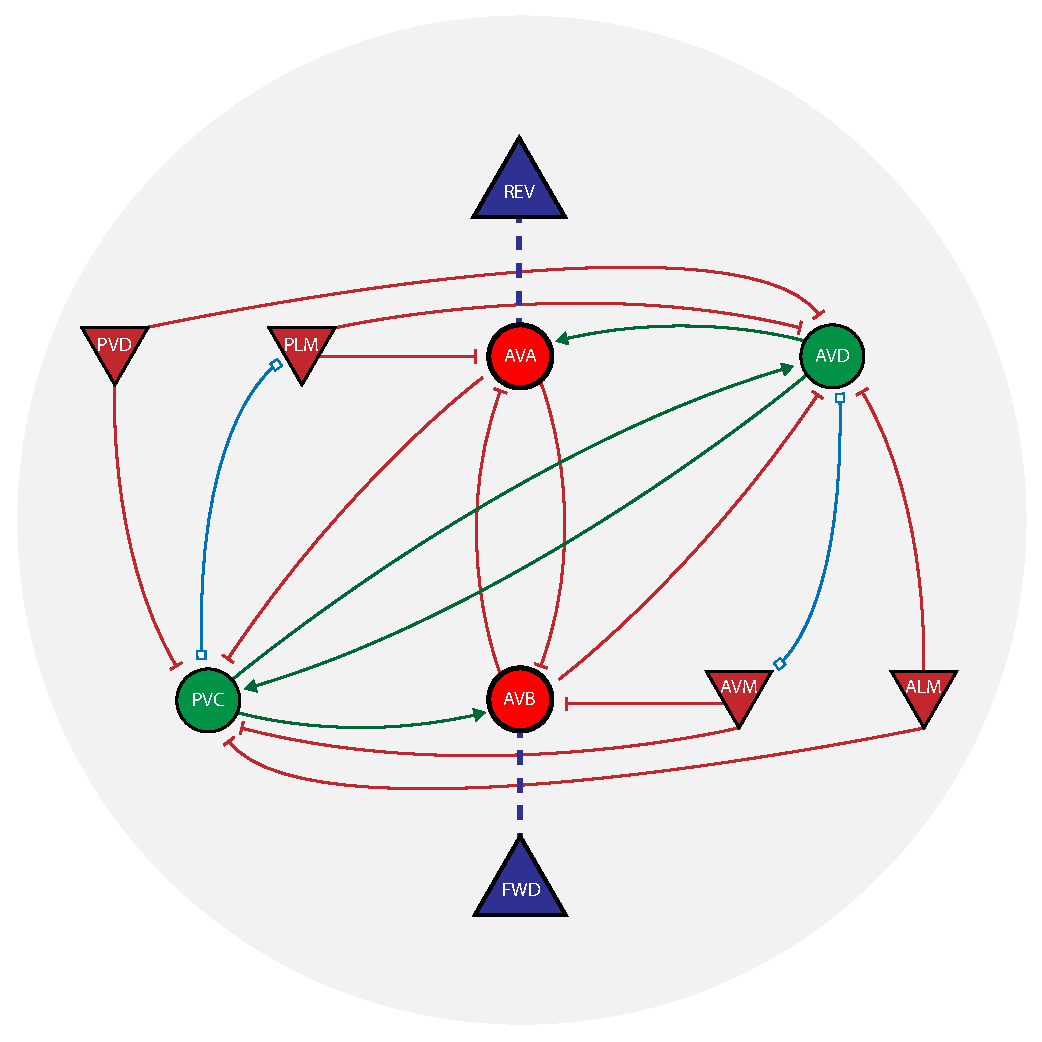
\includegraphics[width=4.5cm]{figures/folie_1/bnn.pdf}\\
			\btEmph{Biologische neuronale Netze}
		\end{column}
		\hspace{0.2cm}
		\begin{column}{0.45\textwidth}
			\vspace{0.8cm}
			\begin{itemize}
				\item[\IconArrow] Nervenzellen \& Synapsen\vspace{0.6cm}
				\item[\IconArrow] Biologisches neuronales Netzwerk\vspace{0.6cm}
				\item[\IconArrow] Symmetrisches neuronales Netzwerk
			\end{itemize}
		\end{column}
	\end{columns}
\end{frame}

% =======================

\begin{frame}
	\frametitle{\ChapterBnn}
	\framesubtitle{Biologische Nervenzellen}
	\vspace{0.3cm}
	\begin{itemize}
		\item Neuronale Netze biologischer Lebensformen bestehen aus Nervenzellen und Synapsen bzw. Gap-Junctions
		\item Neuronale Nervenzellen bestehen aus Dendrit, Soma und Axon. Das Soma enthält den Zellkern und verarbeitet ankommende Informationen.
		\item Der Dendrit dient der Reizaufnahme von Signalen anderer Nervenzellen übertragen durch Synapsen und Gap-Junctions.
		\item Das Axon ist ein Nervenzellenfortsatz zur Weiterleitung der Signale von Soma an weitere Synapsen und Gap-Junctions.
	\end{itemize}
	\begin{figure}[H] %[!t] ...
		\centering
		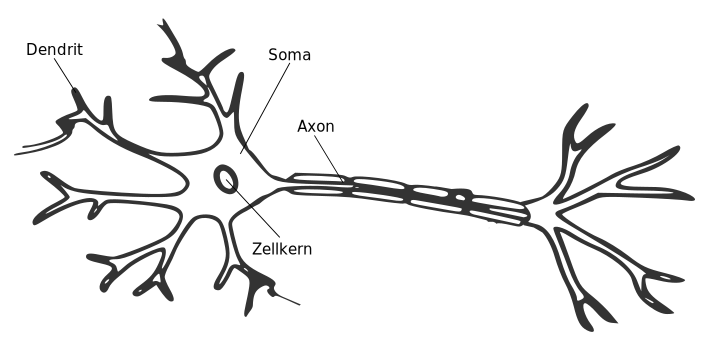
\includegraphics[width=7cm]{figures/folie_2/neuron_is.pdf}
		\label{fig:neuron}
	\end{figure}

\end{frame}

% =======================

\begin{frame}
	\frametitle{\ChapterBnn}
	\framesubtitle{Biologische Synapsen}
	\vspace{0.3cm}
	Eine Synapse dient der Informationsübertragung zwischen zwei Nervenzellen und wird in drei Kategorien unterteilt:
	\begin{itemize}
		\item Exzitatorische Synapsen (chemisch) - wirken anregend auf die postsynaptische Nervenzelle und übertragen die Informationen.
		\item Inhibitorische Synapse (chemisch) - wirken  hemmend auf die postsynaptische Nervenzelle und übertragen die Informationen negativ.
		\item Gap-Junctions (elektrisch) - wirken bidirektional als synchronisierende Verbindung und gleichen Potentialunterschiede aus.
	\end{itemize}
	\begin{figure}[H] %[!t] ...
		\centering
		\includegraphics[width=8cm]{figures/folie_3/synapse_is.pdf}
		\label{fig:synapse}
	\end{figure}

\end{frame}

% =======================

\begin{frame}
	\frametitle{\ChapterBnn}
	\framesubtitle{Biologisches neuronales Netz des \textit{C. Elegans}}
	\vspace{0.3cm}
	Der \textit{Touch-Withdrawal Circuit} des \textit{C. Elegans} dient des reflexartigen Zurückschnellens bei äußeren Stimuli.
	\begin{columns}[T,onlytextwidth]
		\begin{column}{0.55\textwidth}
			\begin{itemize}
				\item[\MotorNeuron] \textbf{Motor-Neuronen} sorgen für die Anregung von Muskelgruppen, um bspw. eine Vorwärtsbewegung umzusetzen.\vspace{0.3cm}
				\item[\SensorNeuron] \textbf{Sensor-Neuronen} nehmen Signale durch äußere Stimuli auf und übersetzen diese auf Aktions-\\potentiale innerhalb des neuronalen Netzes.\vspace{0.3cm}
				\item[\InterNeuron] \textbf{Inter-Neuronen} nehmen durch Synapsen und Gap-Junctions Akionspotentiale entgegen und summieren diese auf, bis ein Schwellwert erreicht wird - das Inter-Neuron feuert.
			\end{itemize}
		\end{column}
		\hspace{0.2cm}
		\begin{column}{0.45\textwidth}
			\vspace{-0.7cm}
			\begin{figure}[H] %[!t] ...
				\centering
				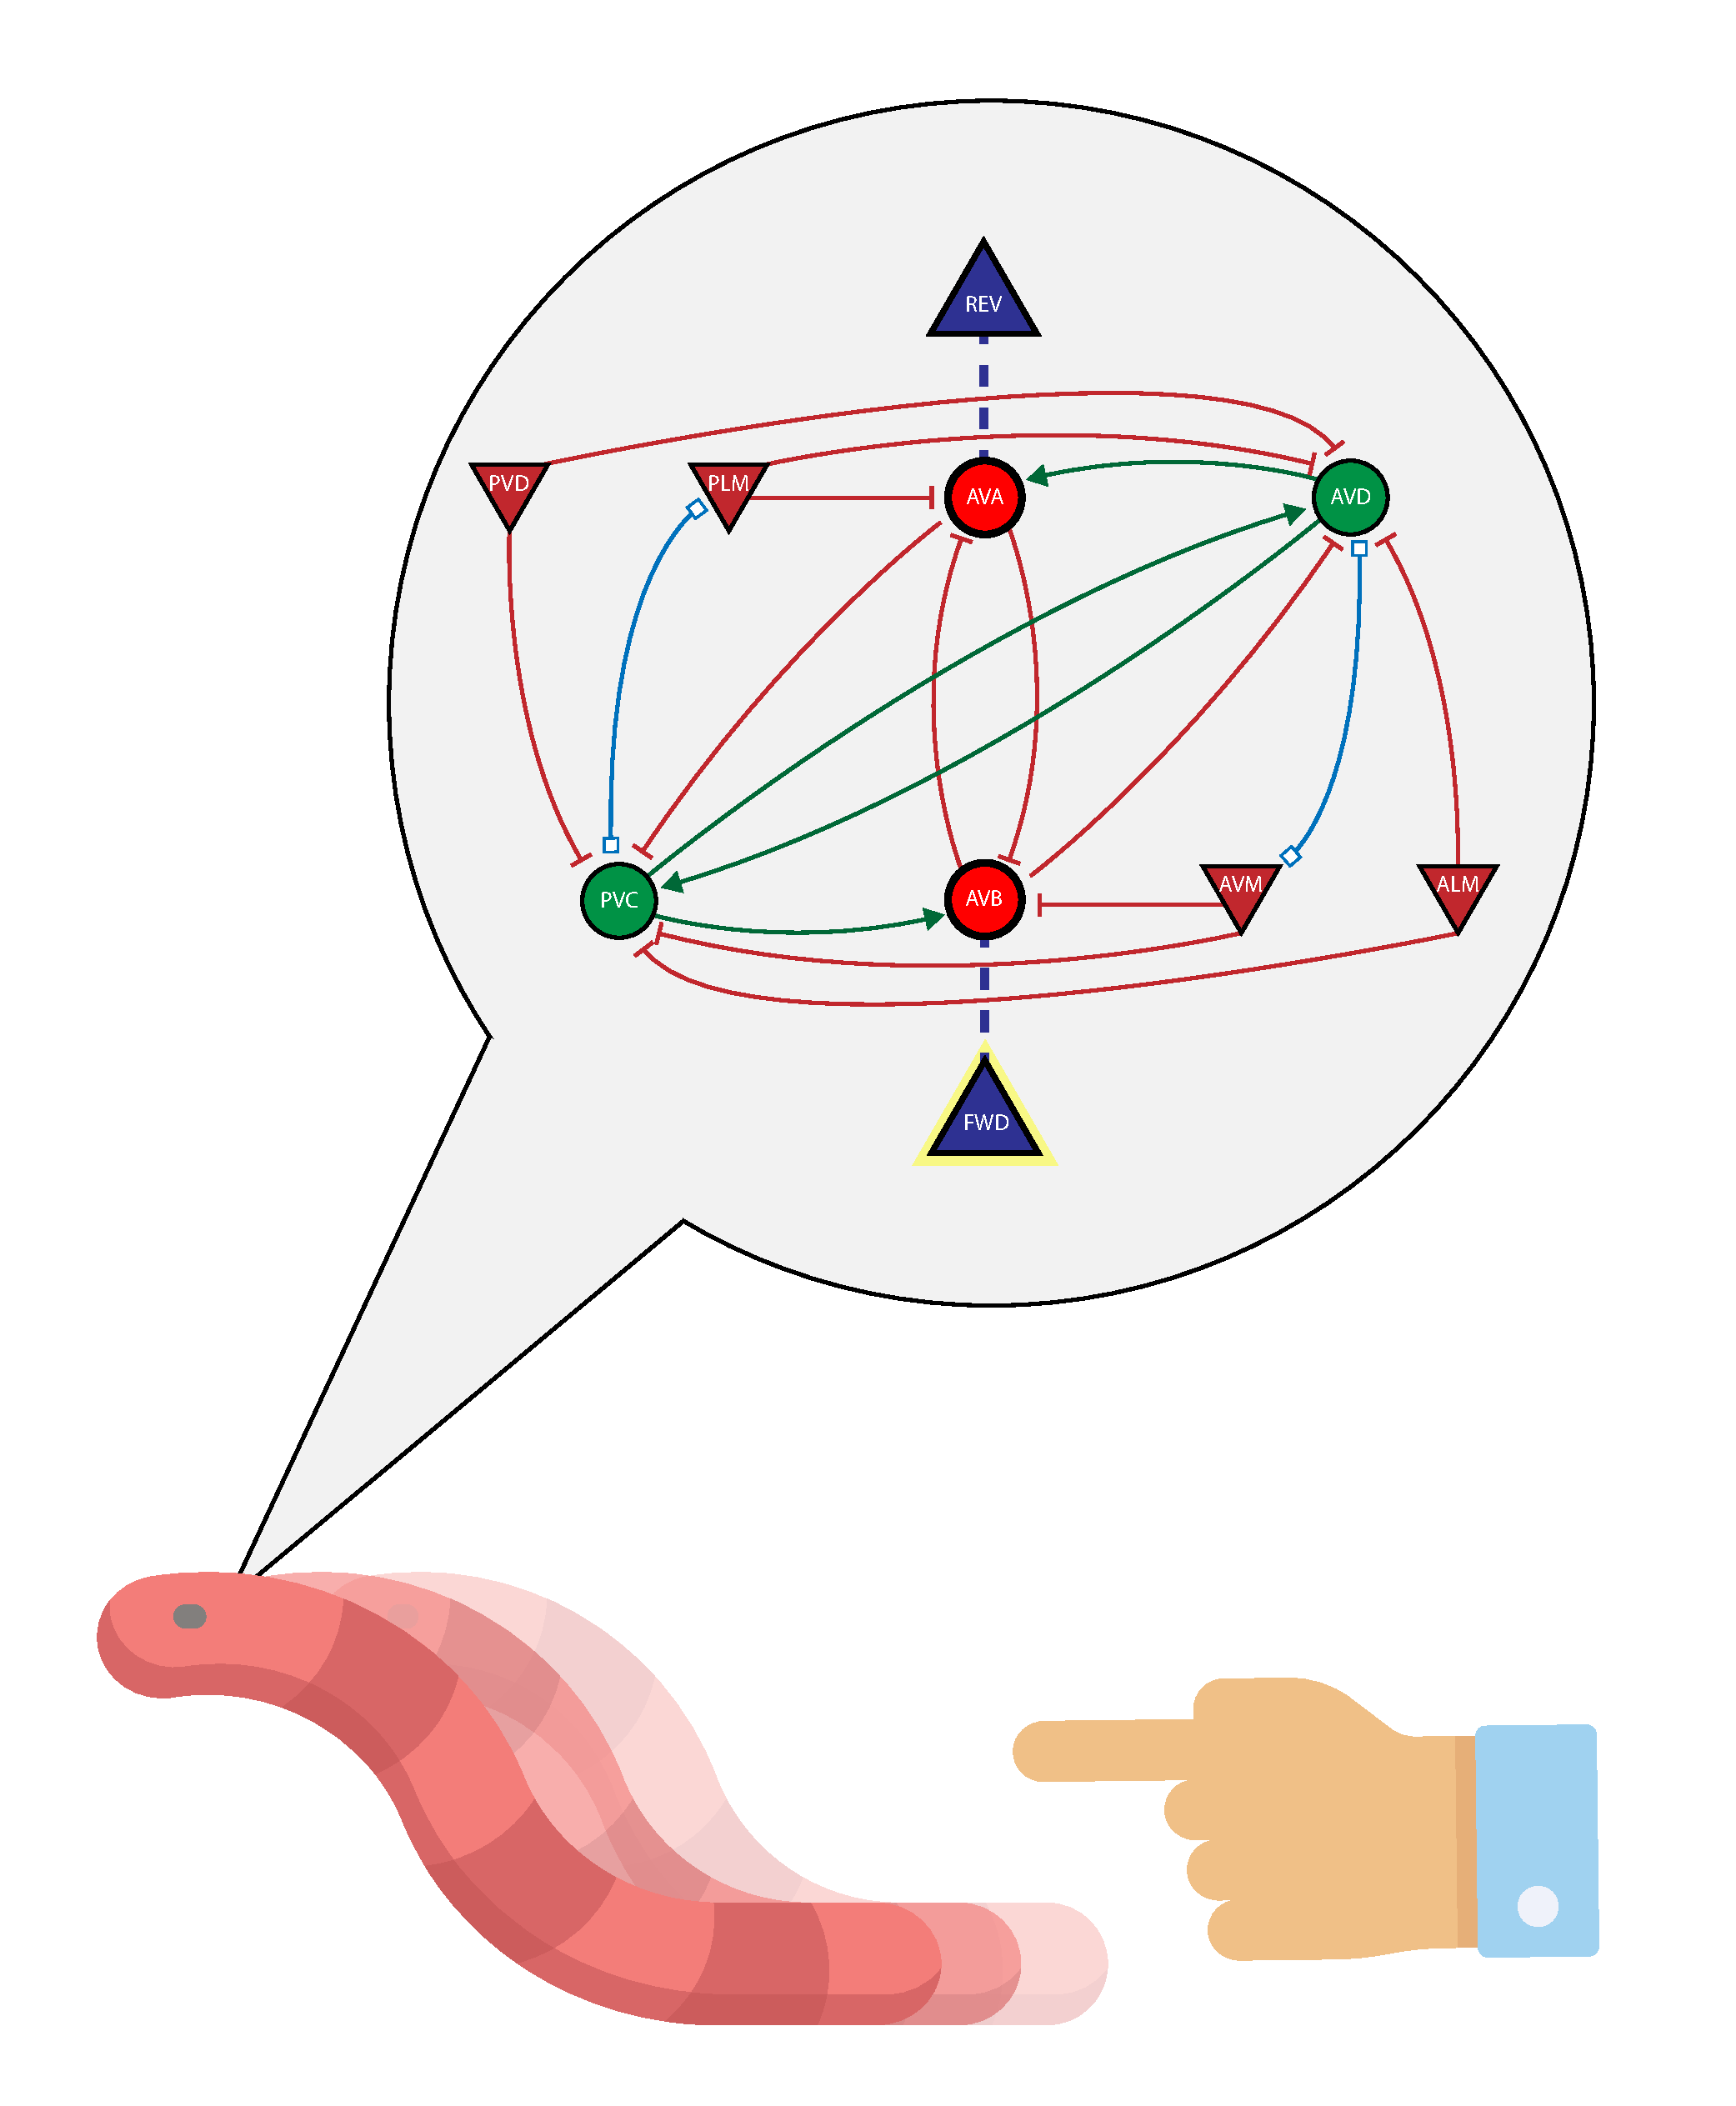
\includegraphics[width=5.5cm]{figures/nn_with_worm.pdf}
				\label{fig:symm_nn}
			\end{figure}
		\end{column}
	\end{columns}
\end{frame}

% =======================

\begin{frame}
	\frametitle{\ChapterBnn}
	\framesubtitle{Neuronale Dynamik durch das Leaky Integrate and Fire - Modell}
	\vspace{0.3cm}
	Die neuronale Dynamik und die damit verbundenen Vorgänge im neuronalen Netz werde durch das Leaky Integrate and Fire (LIF) - Modell dargestellt.
	\begin{columns}[T,onlytextwidth]
		\begin{column}{0.55\textwidth}
			\vspace{0.1cm}
			\begin{alignbox}{0.9\textwidth}
				Berechnung des Membranpotentials bei anliegenden Synapsen- und Gap-Junction-Strömen:\\
				\begin{align}
					\label{eq:lif}
					\frac{dU}{dt} &= \frac{G_{Leak}(U_{Leak} - U) + I_{in}}{C_m}\text{ mit}\\
					\label{eq:lif_current_in}
					I_{in} &= \sum_{i = 1}^{n}{I_{Stimuli}} + \sum_{i = 1}^{n}{I_{Syn}} + \sum_{i = 1}^{n}{I_{Gap}}\text{.}
				\end{align}
			\end{alignbox}\\
			\vspace{0.3cm}
			\begin{alignbox}{0.9\textwidth}
				Berechnung der Synapsen- und Gap-Junction-Ströme:\\	
				\begin{align}
					\label{eq:chem_syn_current}
					I_{Syn} &= \frac{\omega}{1 + \exp^{\sigma(u_{pre} + \mu)}}(E - u_{post}),\\
					\label{eq:gap_syn_current}
					I_{Gap} &= \hat{\omega}(u_{post} - u_{pre})\text{.}
				\end{align}
			\end{alignbox}
		\end{column}
		\hspace{0.2cm}
		\begin{column}{0.45\textwidth}
			\vspace{0.5cm}
			\begin{figure}
				\centering
				\begin{circuitikz}
					\draw
					(0,4) to [short, o-*] (1,4)
					to [generic, l=$R$] (1,2)
					to [battery1, l=$U_{Leak}$] (1,0)
					to [short, -*] (1,0)
					to [short, -o] (0,0)
					
					(1,4) to [short, i_>=$I$] (3,4)
					to [short, -*] (3,4)
					to [C, l=$C_m$] (3,0)
					to [short, -*] (3,0)
					to [short, -*] (1,0)
					
					(3,4) to [short, -o] (4,4)
					(3,0) to [short, -o] (4,0)
					(4,0) to [open, v_<=$U$] (4,4);
				\end{circuitikz}
				\caption{Ersatzschaltbild der Zellmembran}
				\label{cic:lif}
			\end{figure}
		\end{column}
	\end{columns}
\end{frame}

% =======================

\begin{frame}
	\frametitle{\ChapterBnn}
	\framesubtitle{Motivation: Nutzung eines biologischen neuronalen Netzes}
	\vspace{0.5cm}
	Klassische Anwendungen neuronaler Netze stützen sich auf künstlich erstellte Konstrukte, welche durch 
	\vspace{0.5cm}
	\begin{columns}[T,onlytextwidth]
		\begin{column}{0.45\textwidth}
			\begin{itemize}
				\item[\IconPro] Profitieren von natürlicher Evolution.\vspace{0.5cm}
				\item[\IconPro] Starke Anpassungsfähigkeit durch zwei Eingängen und einem Ausgang.\vspace{0.5cm}
				\item[\IconPro] Einfache Erweiterbarkeit und Ausbau des Netzwerks durch Lernalgorithmen.\vspace{0.5cm}
				\item[\IconPro] Kurze Trainingsphasen.\vspace{0.5cm}
			\end{itemize}
		\end{column}
		\hspace{0.2cm}
		\begin{column}{0.45\textwidth}
			\begin{itemize}
				\item[\IconCon] Implementationsaufwand und Simulation aufwendig.\vspace{0.5cm}
				\item[\IconCon] Wenig Fachliteratur über die Verbindung von biologischen neuronalen Netzen mit Methoden des Reinforcement Learning.\vspace{0.5cm}
				\item[\IconCon] Hohe Anzahl an zu simulierenden Parametern.\vspace{0.5cm}
			\end{itemize}
		\end{column}
	\end{columns}

\end{frame}

% =======================

\begin{frame}
\frametitle{\Inhalt}
\vspace{1cm}
\begin{columns}[T,onlytextwidth]
	\begin{column}{0.45\textwidth}
		\centering
		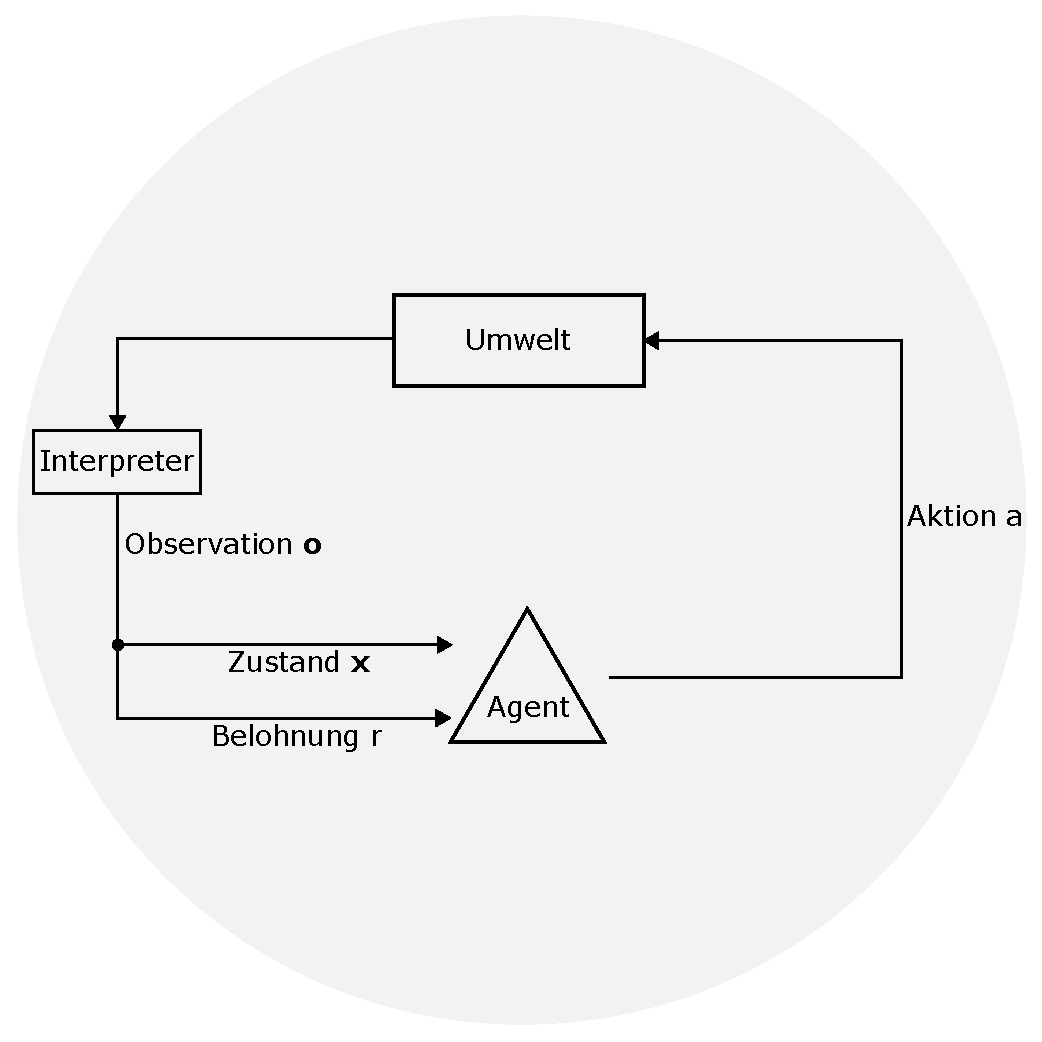
\includegraphics[width=4.5cm]{figures/folie_1/rl.pdf}\\
		\btEmph{Reinforcement Learning}
	\end{column}
	\hspace{0.2cm}
	\begin{column}{0.45\textwidth}
		\vspace{0.4cm}
		\begin{itemize}
			\item[\IconArrow] Deep Learning und Grundlagen von Lernalgorithmen\vspace{0.6cm}
			\item[\IconArrow] Vorteile des Belohnungssystems\vspace{0.6cm}
			\item[\IconArrow] Reinforcement Learning durch Random-Search und genetischen Algorithmen
		\end{itemize}
	\end{column}
\end{columns}
\end{frame}

% =======================

\begin{frame}
	\frametitle{\ChapterRl}
	\framesubtitle{Reinforcement Learning und das Belohnungssystem}
	\vspace{0.3cm}
	\textit{Reinforcement Learning} aus dem Bereich des \textit{Deep Learning} ist eine Abwandlung des überwachten Lernens mit der Erweiterung eines Belohnungssystems.
	\begin{columns}[T,onlytextwidth]
		\begin{column}{0.5\textwidth}
			\begin{itemize}
			  \item Der Agent ist in der Lage, eine Aktion im gegebenen Aktionsraum zu tätigen.
			  \item Die Aktion hat Auswirkungen auf die Umwelt bzw. Simulation, der neue Zustand der Simulation wird interpretiert und als Observationsvektor $\boldsymbol{o}$ ausgegeben.
			  \item Aus der Observation $\boldsymbol{o}$ gehen zum einen der Zustandsvektor $\boldsymbol{x}$ zum anderen die Belohnung $r$ hervor.
			  \item Diese Größen werden von dem Agenten interpretiert und dienen als neue Entscheidungsgrundlage der nächsten Aktion.
			\end{itemize}
		\end{column}
		\hspace{-0.5cm}
		\begin{column}{0.45\textwidth}
			\vspace{1cm}
			\begin{figure}[H] %[!t] ...
				\centering
				\includegraphics[width=8cm]{figures/RL_Chart_pres.pdf}
				\caption{Ablaufplan: \textit{Reinforcement Learning}}
				\label{fig:rl}
			\end{figure}
		\end{column}
	\end{columns}
\end{frame}

% =======================

\begin{frame}
	\frametitle{\ChapterRl}
	\framesubtitle{Anwendung auf das biologische Netzwerk}
	\vspace{0.3cm}
	Durch \textit{Reinforcement Learning} können Parameter im biologischen neuronalen Netz optimiert werden, sodass es zu Feuer-Events kommt.
	\begin{itemize}
		\item Um die neuronale Dynamik durch das \textit{LIF}-Modell richtig abzubilden, damit es bei äußeren Stimuli zu Feuer-Ereignissen kommt, werden insgesamt 46 Parameter simuliert.
		\item ...
		\item Durch verschiedene Suchalgorithmen können Parametersätze simuliert und die Performance gemessen werden.
	\end{itemize}
\end{frame}

% =======================

\begin{frame}
	\frametitle{\ChapterRl}
	\framesubtitle{Suchalgorithmen}
	\vspace{0.3cm}
	\begin{columns}[T,onlytextwidth]
		\begin{column}{0.5\textwidth}
			\btEmph{\texttt{Random-Search}}
			\begin{itemize}
				\item Parameter werden in einer gegebenen Gleichverteilung mit festen Grenzen pro Episode zufällig generiert.
				\item Die Performance jedes Parametersatzes wird anhand der erhaltenen Belohnung gemessen.
				\item Nach Ablauf der Simulationszeit werden diejenigen Parameter gespeichert, welche die höchste Belohnung erhalten haben.
			\end{itemize}
		\end{column}
		\begin{column}{0.5\textwidth}
			\btEmph{\texttt{Weights}}
			\begin{itemize}
				\item Im Gegensatz zu Random-Search wird Weights zur Optimierung des neuronalen Netzes mit bereits bestehenden Parametern verwendet.
				\item Es werden bestehende Synapsen mit einem pro Episode zufällig gewählten Gewicht versehen, welches die Reizübertragung schwächt.
			\end{itemize}
		\end{column}
	\end{columns}
\end{frame}

% =======================

\begin{frame}
\frametitle{\ChapterRl}
\framesubtitle{Suchalgorithmen}
\vspace{0.3cm}
\begin{columns}[T,onlytextwidth]
	\begin{column}{0.5\textwidth}
		\btEmph{\texttt{Genetische Algorithmen}}
		\begin{itemize}
			\item Die erste Generation an Parametern wird in einer gegebenen Gleichverteilung mit festen Grenzen pro Episode zufällig generiert.
			\item Nach Durchlauf der ersten Generation werden wenige Episoden mit guter Belohnung in eine Selektion aufgenommen.
			\item Die Grenzen der Gleichverteilung werden entsprechend der Maxima/Minima der Selektion angepasst.
			\item Die Simulation konvergiert auf ein lokales Maximum für jeden Parameter.
		\end{itemize}
	\end{column}
	\begin{column}{0.45\textwidth}
		\begin{figure}[H] %[!t] ...
			\centering
			\scriptsize
			\def\svgwidth{6.3cm}
			\input{figures/gen_alg.pdf_tex}
			\caption{Grafische Darstellung des genetischen Algorithmus.}
			\label{fig:gen_alg}
		\end{figure}
	\end{column}
\end{columns}
\end{frame}

% =======================


\begin{frame}
\frametitle{\Inhalt}
\vspace{1cm}
\begin{columns}[T,onlytextwidth]
	\begin{column}{0.45\textwidth}
		\centering
		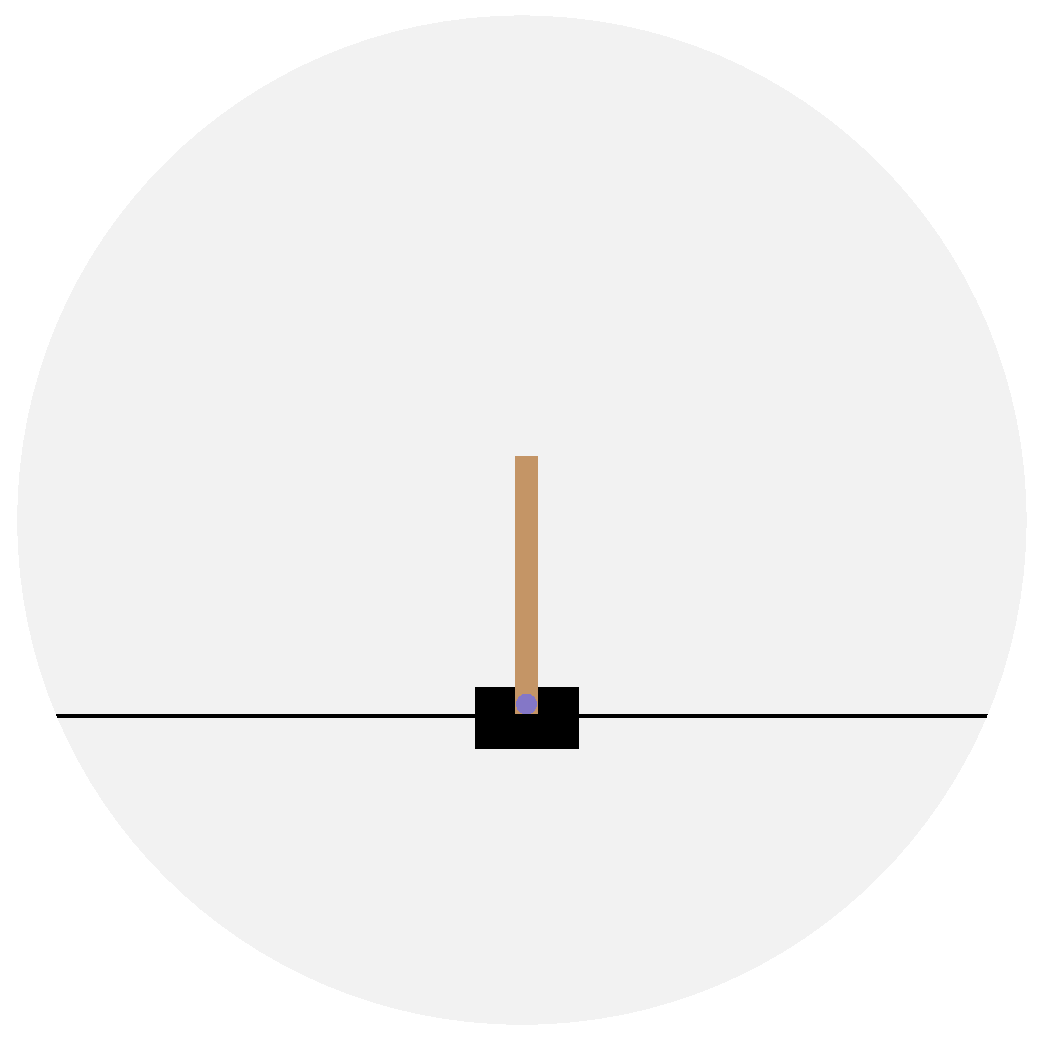
\includegraphics[width=4.5cm]{figures/folie_1/cartpole.pdf}\\
		\btEmph{Simulation: inverses Pendel}
	\end{column}
	\hspace{0.2cm}
	\begin{column}{0.45\textwidth}
		\vspace{0.8cm}
		\begin{itemize}
			\item[\IconArrow] Implementiertung des Simulators\vspace{0.6cm}
			\item[\IconArrow] Simulationsumgebung: OpenAI Gym\vspace{0.6cm}
			\item[\IconArrow] Grafische Darstellung und Auswertung der Simulation
		\end{itemize}
	\end{column}
\end{columns}
\end{frame}

% =======================



\begin{frame}
\frametitle{\ChapterCartpole}
\framesubtitle{Aufbau des Simulators}
\vspace{0.3cm}
\begin{columns}[T,onlytextwidth]
	\begin{column}{0.7\textwidth}
		Um die neuronale Dynamik des biologischen neuronalen Netzes zu simulieren und die Aktionen auf die Umwelt zu übertragen, wurde ein Simulator in der Programmiersprache \texttt{Python} geschrieben.
		\begin{itemize}
			\item ...
		\end{itemize}
	\end{column}
	\hspace{-0.8cm}
	\begin{column}{0.28\textwidth}
		\vspace{-0.7cm}
		\resizebox{4cm}{!} {
		\begin{forest}
			pic dir tree,
			where level=0{}{% folder icons by default; override using file for file icons
				directory,
			},
			[TW Circuit
			[docs]
			[information]
			[modules
			[genetic\_algorithm.py, file]
			[inspect.py, file]
			[lif.py, file]
			[parameters.py, file]
			[random\_search\_v2.py, file]
			[visiualize.py, file]
			[weights.py, file]]
			[parameter\_dumps]
			[weight\_dumps]
			[main.py, file]]
		\end{forest}
		}
	\end{column}
\end{columns}
\end{frame}

% =======================

\begin{frame}
\frametitle{\ChapterCartpole}
\framesubtitle{Simulationsumgebung \texttt{CartPole\_v0}}
\vspace{0.3cm}
Um die Methode des \textit{Reinforcement Learning} auf biologische neuronale Netze anzuwenden, wird die Simulationsumgebung \texttt{CartPole\_v0} von OpenAi Gym gewählt.
\begin{columns}[T,onlytextwidth]
	\begin{column}{0.53\textwidth}
		\begin{itemize}
			\item Das inverse Pendel auf dem Wagen kann sich in Vorwärts- und Rückwärtsrichtung bewegen.
			\item Pro Zeitschritt kann ein Schritt in die jeweilige Richtung erfolgen (Aktion: 0 oder 1).
			\item Der Observationsvektor $\boldsymbol{o}$ gibt die Zustandsgrößen $\varphi$, $\dot{\varphi}$, $x$ und $\dot{x}$ wieder.
			\item Es wird ebenfalls eine Belohnung $r$ zurückgegeben.
			\item ...
		\end{itemize}
	\end{column}
	\hspace{-0.5cm}
	\begin{column}{0.45\textwidth}
		\vspace{-0.6cm}
		\begin{figure}[H] %[!t] ...
			\centering
			\scriptsize
			\def\svgwidth{6.5cm}
			\input{figures/cartpole_with_ann.pdf_tex}
			\caption{Simulationsumgebung \texttt{CartPole\_v0}}
			\label{fig:cartpole}
		\end{figure}
	\end{column}
\end{columns}
\end{frame}

% =======================

\begin{frame}
	\frametitle{\ChapterCartpole}
	\framesubtitle{Simulationsläufe: Auslagerung auf Cloud Server}
	\vspace{0.3cm}
	\begin{itemize}
		\item Durch rechenintensive Simulationen mit den Algorithmen \texttt{Random-Search} und \texttt{Weights} wird ein externer Server benötigt.
		\item Eine virtuelle Instanz in der Google Cloud Platform wurde angemietet, um Simulationszeiten über 12 Stunden zu ermöglichen.
		\item Es wurden Simulationen mit über 10 Mio. Episoden gefahren und analysiert.
		\item ...
	\end{itemize}
	\begin{figure}[H] %[!t] ...
		\centering
		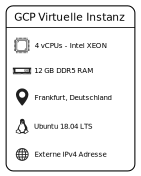
\includegraphics[width=8cm]{figures/gcp.png}
		\label{fig:gcp}
	\end{figure}

\end{frame}

% =======================

\begin{frame}
	\frametitle{\ChapterCartpole}
	\framesubtitle{Visualisierung der Simulationsergebnisse}
	\vspace{0.3cm}
	\begin{itemize}
		\item ...
	\end{itemize}

\end{frame}

% =======================

\begin{frame}
	\frametitle{\ChapterCartpole}
	\framesubtitle{Simulation des inversen Pendels (Video)}
	\vspace{0.3cm}
	Das Video zeigt das inverse Pendel, welches durch das biologische neuronale Netz und bereits trainierten Parametern stabilisiert wird.\\
	\vspace{0.3cm}
		\centering
		\vspace{0.5cm}
		\includemedia[
		width=14cm,height=6cm,
		activate=pageopen,
		addresource=video/20180910_Render_MP4.mp4,
		flashvars={
			source=video/20180910_Render_MP4.mp4
			&autoPlay=true
		}
		]{}{VPlayer.swf}

\end{frame}

% =======================

\begin{frame}
	\frametitle{\ChapterEnd}
	\framesubtitle{Zusammenfassung \& Ausblick}
	\vspace{0.3cm}
	\begin{itemize}
		\item ...
	\end{itemize}

\end{frame}

% =======================

\begin{frame}[c]
	\frametitle{\ChapterEnd}
	\centering
	{\LARGE Vielen Dank für Ihre Aufmerksamkeit.}

\end{frame}

% =======================

\begin{frame}
  \frametitle{Formatting text}
  \framesubtitle{Color and thickness}

  \begin{itemize}
  \item Emphasizing text  cell
    \begin{itemize}
    \item \texttt{\textbackslash cEmph} provides \cEmph{this text}
    \item \texttt{\textbackslash ctEmph} provides \ctEmph{this text}
    \item \texttt{\textbackslash tEmph} provides \tEmph{this text}
    \item \texttt{\textbackslash bEmph} provides \bEmph{this text}
    \item \texttt{\textbackslash btEmph} provides \btEmph{this text}
    \end{itemize}
  \end{itemize}  
\end{frame}

% =======================

\begin{frame}[fragile]
  \frametitle{Boxes}
  \framesubtitle{Some examples}

\begin{verbatim}
\begin{displaybox}{0.995\textwidth}
  Example 1: use 0.995\textbackslash textwidth for full width box  
\end{displaybox}
\end{verbatim}
  
  \begin{displaybox}{0.995\textwidth}
    % 
    Example 1: use 0.995\textbackslash textwidth for full width box 
    % 
  \end{displaybox}
  
\begin{verbatim}
\begin{alignbox}{0.75\textwidth} 
  Use for math related environments including text line (blank line below)

  \begin{align}
    y = x^2
  \end{align}
\end{alignbox}
\end{verbatim}
  
  \begin{alignbox}{0.75\textwidth}
    Use for math related environments including text line (blank line below)
    
    \begin{align}
      y = x^2
    \end{align}
  \end{alignbox}
  %
\end{frame}

% =======================

\begin{frame}[fragile,fragile]
  \frametitle{Boxes}
  \framesubtitle{Some examples}
  
\begin{verbatim}
\begin{alignbox}{0.5\textwidth} 
  \begin{align}
    y = x^2
  \end{align}
\end{alignbox}
\end{verbatim}
  
  \begin{alignbox}{0.5\textwidth}
    \begin{align}
      y = x^2
    \end{align}
  \end{alignbox}
  %

\begin{verbatim}
This shows the use of an \texttt{inlinebox} environment
\begin{inlinebox}{1cm}
  abc
\end{inlinebox}
\end{verbatim}\newenvironment{onlinebox}[1]

This shows the use of an \texttt{inlinebox} environment
\begin{inlinebox}{1cm}
  abc
\end{inlinebox}

\end{frame}

% =======================

\begin{frame}\frametitle{Differenzielle Flachheit}
  \framesubtitle{Inversionsbasierte Trajektorienplanung}
  %
  \newcommand{\pfeil}{\VECTOR(0,0)(3,0)}
  \newcommand{\kasten}{\polyline(0,0)(4,0)(4,3)(0,3)(0,0)}
  %
  \begin{itemize}
  \item \btEmph{Differenzielle Flachheit}\sfcite{fliess:95}
    \medskip
    \begin{inlinebox}{0.925\textwidth}
      Ein System $\dot{\xv[]}=\bs{f}(\xv[],\uv[])$ wird \tEmph{differenziell
        flach} genannt, wenn ein so genannter \tEmph{flacher Ausgang}
      $\yv[]=\bs{h}(\xv[],\uv[])$, $\dim\yv[]=\dim\uv[]$ existiert, so dass \\[1ex]
      % 
      \phantom{-----} 
      $\xv =
      \bs{\theta_{\xv[]}}\Bigl(\yv[],\dot{\yv[]},\ldots,\yv[^{(\beta)}]\Bigr)$,
      \qquad 
      $\uv =
      \bs{\theta_{\uv[]}}\Bigl(\yv[],\dot{\yv[]},\ldots,\yv[^{(\beta+1)}]\Bigr)$.
    \end{inlinebox}
    %
    $\Rightarrow$ \tEmph{Differenzielle Zustands-- und
      Eingangsparametrierung} \pause\\[-1ex]
    % 
    \unitlength0.5cm
    \begin{picture}(26,4)(0,1.25)
      \linethickness{1.25pt}
      \put(1,0){%
        \put(10,3){\pfeil}
        \put(13,1.5){\kasten}
        \put(13.75,2.75){System}
        \put(17,3){\pfeil}
        % 
        \put(17.5,3.5){$\xv[\cts]\to\cEmph{\xvd[\cts]=\bs{\theta_{\xv[]}}\bigl(\yvd[],\dot{\yvd[]},...\bigr)}$}
      }
      %
      \put(3,3){\cEmph{\pfeil}}
      \put(6,1.5){\cEmph{\kasten}}
      \put(10,3){\Line(0,0)(0,0)(1,0)}
      \put(6.15,2.75){$\bs{\theta}_{\uv[]}\bigl(\yvd[],\!\dot{\yvd[]}\!,...\bigr)$}
      \put(10.1,3.5){$\cEmph{\uvd}=\uv$}
      \put(3.25,3.5){\cEmph{$\yvd$}}
    \end{picture}\pause\\
    %
    $\Rightarrow$ Methodische \"Ubertragung auf
    \tEmph{verteilt--parametrische Systeme}
  \end{itemize}
  % 
\end{frame}

% =======================

\ClosingSlide

\end{document}

%%% Local Variables:
%%% mode: latex
%%% TeX-master: t
%%% End:
